%%%%%%%%%%%%%%%%%%%%%%%%%%%%%%%%%%%%%%%%
% datoteka diplomska_naloga.tex
%
% DIPLOMSKA NALOGA: Porazdeljeno upodabljanje v spletu
% Avtor: Luka Prijatelj
% 
%%%%%%%%%%%%%%%%%%%%%%%%%%%%%%%%%%%%%%%%

\documentclass[a4paper, 12pt, tikz, border=5]{book}
%\documentclass[a4paper, 12pt, draft]{book}  Nalogo preverite tudi z opcijo draft, ki vam bo pokazala, katere vrstice so predolge!

\usepackage[utf8x]{inputenc}   % omogoča uporabo slovenskih črk kodiranih v formatu UTF-8
\usepackage[slovene,english]{babel}    % naloži, med drugim, slovenske delilne vzorce
\usepackage[pdftex]{graphicx}  % omogoča vlaganje slik različnih formatov
\usepackage{fancyhdr}          % poskrbi, na primer, za glave strani
\usepackage{amssymb}           % dodatni simboli
\usepackage{amsmath}           % eqref, npr.
%\usepackage{hyperxmp}
\usepackage[hyphens]{url}  
\usepackage{comment}      
\usepackage{listings}
\usepackage{forest}

% TODO: TE SPODNJE VRSTICE SEM DODAL, ZA TABELO GENERATORJEV/JEZIKOV
\usepackage{graphicx}
\usepackage{caption}
\usepackage{booktabs}
\usepackage{array}
\newcommand*\rotbf[1]{\rotatebox{90}{\textbf{#1}}}
\newcommand{\specialcell}[2][c]{\begin{tabular}[#1]{@{}l@{}}#2\end{tabular}}


\usepackage[pdftex, colorlinks=true,
						citecolor=black, filecolor=black, 
						linkcolor=black, urlcolor=black,
						pagebackref=false, 
						pdfproducer={LaTeX}, pdfcreator={LaTeX}, hidelinks]{hyperref}
\usepackage{color}     
\usepackage{soul}      
\usepackage{tikz}

% max depth that table of contents can show
\addtocontents{toc}{\setcounter{tocdepth}{5}}

%%%%%%%%%%%%%%%%%%%%%%%%%%%%%%%%%%%%%%%%
%	DIPLOMA INFO
%%%%%%%%%%%%%%%%%%%%%%%%%%%%%%%%%%%%%%%%
% Todo: check if titles are ok!
\newcommand{\ttitle}{Porazdeljeno upodabljanje v spletu}
\newcommand{\ttitleEn}{Web-based distributed rendering}
\newcommand{\tsubject}{\ttitle}
\newcommand{\tsubjectEn}{\ttitleEn}
\newcommand{\tauthor}{Luka Prijatelj}
\newcommand{\tkeywords}{Gramatike, Sintakse, Analizatorji, Odprtokodnost}
\newcommand{\tkeywordsEn}{Grammars, Syntax, Analyzer, Open-Source}
\renewcommand{\lstlistingname}{Izvorna koda}



%%%%%%%%%%%%%%%%%%%%%%%%%%%%%%%%%%%%%%%%
%	HYPERREF SETUP
%%%%%%%%%%%%%%%%%%%%%%%%%%%%%%%%%%%%%%%%
\hypersetup{pdftitle={\ttitle}}
\hypersetup{pdfsubject=\ttitleEn}
\hypersetup{pdfauthor={\tauthor, lp0761@student.uni-lj.si}}
\hypersetup{pdfkeywords=\tkeywordsEn}


%%%%%%%%%%%%%%%%%%%%%%%%%%%%%%%%%%%%%%%%
% postavitev strani
%%%%%%%%%%%%%%%%%%%%%%%%%%%%%%%%%%%%%%%%  

\addtolength{\marginparwidth}{-20pt} % robovi za tisk
\addtolength{\oddsidemargin}{40pt}
\addtolength{\evensidemargin}{-40pt}

\renewcommand{\baselinestretch}{1.3} % ustrezen razmik med vrsticami
\setlength{\headheight}{15pt}        % potreben prostor na vrhu
\renewcommand{\chaptermark}[1]%
{\markboth{\MakeUppercase{\thechapter.\ #1}}{}} \renewcommand{\sectionmark}[1]%
{\markright{\MakeUppercase{\thesection.\ #1}}} \renewcommand{\headrulewidth}{0.5pt} \renewcommand{\footrulewidth}{0pt}
\fancyhf{}
\fancyhead[LE,RO]{\sl \thepage} 
%\fancyhead[LO]{\sl \rightmark} \fancyhead[RE]{\sl \leftmark}
\fancyhead[RE]{\sc \tauthor}              
\fancyhead[LO]{\sc Diplomska naloga}    

\newcommand{\BibTeX}{{\sc Bib}\TeX}

%%%%%%%%%%%%%%%%%%%%%%%%%%%%%%%%%%%%%%%%
% naslovi
%%%%%%%%%%%%%%%%%%%%%%%%%%%%%%%%%%%%%%%%  


\newcommand{\autfont}{\Large}
\newcommand{\titfont}{\LARGE\bf}
\newcommand{\clearemptydoublepage}{\newpage{\pagestyle{empty}\cleardoublepage}}
\setcounter{tocdepth}{1}	      % globina kazala

%%%%%%%%%%%%%%%%%%%%%%%%%%%%%%%%%%%%%%%%
% konstrukti
%%%%%%%%%%%%%%%%%%%%%%%%%%%%%%%%%%%%%%%%  
\newtheorem{izrek}{Izrek}[chapter]
\newtheorem{trditev}{Trditev}[izrek]
\newenvironment{dokaz}{\emph{Dokaz.}\ }{\hspace{\fill}{$\Box$}}

%%%%%%%%%%%%%%%%%%%%%%%%%%%%%%%%%%%%%%%%%%%%%%%%%%%%%%%%%%%%%%%%%%%%%%%%%%%%%%%
%% PDF-A
%%%%%%%%%%%%%%%%%%%%%%%%%%%%%%%%%%%%%%%%%%%%%%%%%%%%%%%%%%%%%%%%%%%%%%%%%%%%%%%


%%%%%%%%%%%%%%%%%%%%%%%%%%%%%%%%%%%%%%%% 
% define medatata
%%%%%%%%%%%%%%%%%%%%%%%%%%%%%%%%%%%%%%%% 
\def\Title{\ttitle}
\def\Author{\tauthor, lp0761@student.uni-lj.si}
\def\Subject{\ttitleEn}
\def\Keywords{\tkeywordsEn}

%%%%%%%%%%%%%%%%%%%%%%%%%%%%%%%%%%%%%%%% 
% \convertDate converts D:20080419103507+02'00' to 2008-04-19T10:35:07+02:00
%%%%%%%%%%%%%%%%%%%%%%%%%%%%%%%%%%%%%%%% 
\def\convertDate{%
    \getYear
}

{\catcode`\D=12
 \gdef\getYear D:#1#2#3#4{\edef\xYear{#1#2#3#4}\getMonth}
}
\def\getMonth#1#2{\edef\xMonth{#1#2}\getDay}
\def\getDay#1#2{\edef\xDay{#1#2}\getHour}
\def\getHour#1#2{\edef\xHour{#1#2}\getMin}
\def\getMin#1#2{\edef\xMin{#1#2}\getSec}
\def\getSec#1#2{\edef\xSec{#1#2}\getTZh}
\def\getTZh +#1#2{\edef\xTZh{#1#2}\getTZm}
\def\getTZm '#1#2'{%
    \edef\xTZm{#1#2}%
    \edef\convDate{\xYear-\xMonth-\xDay T\xHour:\xMin:\xSec+\xTZh:\xTZm}%
}

\expandafter\convertDate\pdfcreationdate 

%%%%%%%%%%%%%%%%%%%%%%%%%%%%%%%%%%%%%%%%
% get pdftex version string
%%%%%%%%%%%%%%%%%%%%%%%%%%%%%%%%%%%%%%%% 
\newcount\countA
\countA=\pdftexversion
\advance \countA by -100
\def\pdftexVersionStr{pdfTeX-1.\the\countA.\pdftexrevision}


%%%%%%%%%%%%%%%%%%%%%%%%%%%%%%%%%%%%%%%%
% XMP data
%%%%%%%%%%%%%%%%%%%%%%%%%%%%%%%%%%%%%%%%  
\usepackage{xmpincl}
\includexmp{pdfa-1b}

%%%%%%%%%%%%%%%%%%%%%%%%%%%%%%%%%%%%%%%%
% pdfInfo
%%%%%%%%%%%%%%%%%%%%%%%%%%%%%%%%%%%%%%%%  
\pdfinfo{%
    /Title    (\ttitle)
    /Author   (\tauthor, lp0761@student.uni-lj.si)
    /Subject  (\ttitleEn)
    /Keywords (\tkeywordsEn)
    /ModDate  (\pdfcreationdate)
    /Trapped  /False
}









%%%%%%%%%%%%%%%%%%%%%%%%%%%%%%%%%%%%%%%%%%%%%%%%%%%%%%%%%%%%%%%%%%%%%%%%%%%%%%%
%%%%%%%%%%%%%%%%%%%%%%%%%%%%%%%%%%%%%%%%%%%%%%%%%%%%%%%%%%%%%%%%%%%%%%%%%%%%%%%

\begin{document}
\selectlanguage{slovene}
\frontmatter
\setcounter{page}{1} %
\renewcommand{\thepage}{}       % preprecimo težave s številkami strani v kazalu
\newcommand{\sn}[1]{"`#1"'}                    % (slovenski narekovaji)

%%%%%%%%%%%%%%%%%%%%%%%%%%%%%%%%%%%%%%%%
% NASLOVNICA
 \thispagestyle{empty}%
   \begin{center}
    {\large\sc Univerza v Ljubljani\\%
      Fakulteta za računalništvo in informatiko}%
    \vskip 10em%
    {\autfont \tauthor\par}%
    {\titfont \ttitle \par}%
    {\vskip 3em \textsc{DIPLOMSKO DELO\\[5mm]         % za ostale študijske programe
    UNIVERZITETNI  ŠTUDIJSKI PROGRAM\\ PRVE STOPNJE\\ RAČUNALNIŠTVO IN INFORMATIKA}\par}%
    \vfill\null%
    {\large \textsc{Mentor}: doc.\ dr. Matija Marolt\par}%
    {\large \textsc{Somentor}:  izr.\ prof.\ dr. Ciril Bohak \par}
    {\vskip 2em \large Ljubljana, 2017 \par}%
\end{center}
% prazna stran
%\clearemptydoublepage      % (izjava o licencah itd. se izpiše na hrbtni strani naslovnice)

%%%%%%%%%%%%%%%%%%%%%%%%%%%%%%%%%%%%%%%%
% COPYRIGHT STRAN
\thispagestyle{empty}
\vspace*{8cm}

\noindent
{\sc Copyright}. 
Rezultati diplomske naloge so intelektualna lastnina avtorja in Fakultete za računalništvo in informatiko Univerze v Ljubljani.
Za objavo in koriščenje rezultatov diplomske naloge je potrebno pisno privoljenje avtorja, Fakultete za računalništvo in informatiko ter mentorja.

\begin{center}
\mbox{}\vfill
\emph{Besedilo je oblikovano z urejevalnikom besedil \LaTeX.}
\end{center}
% prazna stran
\clearemptydoublepage

%%%%%%%%%%%%%%%%%%%%%%%%%%%%%%%%%%%%%%%%
% stran 3 med uvodnimi listi
\thispagestyle{empty}
\vspace*{4cm}

\noindent
Fakulteta za računalništvo in informatiko izdaja naslednjo nalogo:
\medskip
\begin{tabbing}
\hspace{32mm}\= \hspace{6cm} \= \kill




Tematika naloge:
\end{tabbing}
Besedilo teme diplomskega dela študent prepiše iz študijskega informacijskega sistema, kamor ga je vnesel mentor. V nekaj stavkih bo opisal, kaj pričakuje od kandidatovega diplomskega dela. Kaj so cilji, kakšne metode uporabiti, morda bo zapisal tudi ključno literaturo.
\vspace{15mm}

\vspace{2cm}


% PRAZNA STRAN ===================================================
\clearemptydoublepage


% ZAHVALA ===================================================
\thispagestyle{empty}\mbox{}\vfill\null\it%
\noindent
%Na tem mestu zapišite, komu se zahvaljujete za izdelavo diplomske naloge. Pazite, da ne boste koga pozabili. Utegnil vam bo zameriti. Temu se da izogniti tako, da celotno zahvalo izpustite.
\rm\normalfont


% PRAZNA STRAN ===================================================
\clearemptydoublepage


%%%%%%%%%%%%%%%%%%%%%%%%%%%%%%%%%%%%%%%%
% POSVETILO (če sama zahvala ne zadošča :) =================================================== 
\thispagestyle{empty}\mbox{}{\vskip0.20\textheight}\mbox{}\hfill\begin{minipage}{0.55\textwidth}%
Družini in prijateljem.
\normalfont\end{minipage}


% PRAZNA STRAN ===================================================
\clearemptydoublepage


%%%%%%%%%%%%%%%%%%%%%%%%%%%%%%%%%%%%%%%%
% KAZALO ===================================================
\pagestyle{empty}
\def\thepage{}% preprecimo tezave s stevilkami strani v kazalu
\tableofcontents{}


% PRAZNA STRAN ===================================================
\clearemptydoublepage


%%%%%%%%%%%%%%%%%%%%%%%%%%%%%%%%%%%%%%%%
% SEZNAM KRATIC ===================================================

\chapter*{Seznam uporabljenih kratic}  % spremenil Solina, da predolge vrstice ne gredo preko desnega roba
% TODO: preglej, ali so res vse kratice tukaj tudi uporabljene v dokumentu/besedilu
\begin{comment}
\begin{tabular}{l|l|l}
  {\bf kratica} & {\bf angleško} & {\bf slovensko} \\ \hline
  {\bf GUI} & Graphical User Interface & Grafični uporabniški vmesnik \\
  {\bf ALL} & Adaptive LL & Prilagodljiv LL \\
  {\bf PEG} & Parsing Expression Grammar & Razčlenjevalno izrazna gramatika \\
  {\bf GCC} & GNU Compiler Collection & GNU zbirka prevajalnikov \\
  {\bf CFG} & Context-Free Grammar & Kontekstno neodvisna gramatika \\
  {\bf DCFG} & Deterministic Context-Free Grammar & Deterministično kontekstno neodvisna gramatika \\
  {\bf YACC} & Yet Another Compiler-Compiler & Še en izdelovalnik prevajalnika \\
  {\bf CFL} & Context-Free Language & Kontekstno neodvisni jezik \\
  {\bf XML} & eXtensible Markup Language & Razširljiv označevalni jezik \\
  {\bf DTD} & Document Type Definition & Definicija tipa dokumenta \\
  {\bf DCFL} & Deterministic Context-Free Language & Deterministično kontekstno neodvisni jezik \\
  {\bf ANTLR} & ANother Tool for Language Recognition & Še eno orodje za razpoznavo jezika \\
  {\bf BNF} & Backus-Naur Form & Backus-Naur oblika \\
  {\bf EBNF} & Extended Backus-Naur Form & Razširjena Backus-Naur oblika \\
  {\bf ABNF} & Augmented Backus-Naur Form & Povečana Backus-Naur oblika \\
  {\bf WSN} & Wirth Syntax Notation & Wirth sintaksna notacija \\
  {\bf DCF} & Definite Clause Grammar & Razločna stavčna gramatika \\
  {\bf LALR} & LookAhead LR & Vnaprejšnji LR \\
  {\bf SLR} & Simple LR & Preprosti LR \\
  {\bf CYK} & Cocke, Younger, Kasami & Cocke, Younger, Kasami \\
  {\bf LL} & Left to right, performing Leftmost derivation & Iz leve v desno izvršujoč najbolj levo izpeljavo \\
  {\bf LL} & Left to right, performing Rightmost derivation & Iz leve v desno izvršujoč najbolj desno izpeljavo \\
  {\bf GLR} & Generalized LR & Posplošeni LR \\
  \dots & \dots & \dots \\
\end{tabular}
\end{comment}

\noindent\begin{tabular}{p{0.1\textwidth}|p{.4\textwidth}|p{.4\textwidth}}    % po potrebi razširi prvo kolono tabele na račun drugih dveh!
  {\bf kratica} & {\bf angleško} & {\bf slovensko} \\ \hline
  {\bf GUI} & Graphical User Interface & Grafični uporabniški vmesnik \\
  {\bf ALL} & Adaptive LL & Prilagodljiv LL \\
  {\bf PEG} & Parsing Expression Grammar & Razčlenjevalno izrazna gramatika \\
  {\bf GCC} & GNU Compiler Collection & GNU zbirka prevajalnikov \\
  {\bf CFG} & Context-Free Grammar & Kontekstno neodvisna gramatika \\
  {\bf DCFG} & Deterministic Context-Free Grammar & Deterministično kontekstno neodvisna gramatika \\
  {\bf YACC} & Yet Another Compiler-Compiler & Še en izdelovalnik prevajalnika \\
  {\bf CFL} & Context-Free Language & Kontekstno neodvisni jezik \\
  {\bf XML} & eXtensible Markup Language & Razširljiv označevalni jezik \\
  {\bf DTD} & Document Type Definition & Definicija tipa dokumenta \\
  {\bf DCFL} & Deterministic Context-Free Language & Deterministično kontekstno neodvisni jezik \\
  {\bf ANTLR} & ANother Tool for Language Recognition & Še eno orodje za razpoznavo jezika \\
  {\bf BNF} & Backus-Naur Form & Backus-Naur oblika \\
  {\bf EBNF} & Extended Backus-Naur Form & Razširjena Backus-Naur oblika \\
  {\bf ABNF} & Augmented Backus-Naur Form & Povečana Backus-Naur oblika \\
  {\bf WSN} & Wirth Syntax Notation & Wirth sintaksna notacija \\
  {\bf DCF} & Definite Clause Grammar & Razločna stavčna gramatika \\
  {\bf LALR} & LookAhead LR & Vnaprejšnji LR \\
  {\bf SLR} & Simple LR & Preprosti LR \\
  {\bf CYK} & Cocke, Younger, Kasami & Cocke, Younger, Kasami \\
  {\bf LL} & Left to right, performing Leftmost derivation & Iz leve v desno izvršujoč najbolj levo izpeljavo \\
  {\bf LL} & Left to right, performing Rightmost derivation & Iz leve v desno izvršujoč najbolj desno izpeljavo \\
  {\bf GLR} & Generalized LR & Posplošeni LR \\ \\
  \dots & \dots & \dots \\
\end{tabular}


% PRAZNA STRAN ===================================================
\clearemptydoublepage


%%%%%%%%%%%%%%%%%%%%%%%%%%%%%%%%%%%%%%%%
% POVZETEK ===================================================
\addcontentsline{toc}{chapter}{Povzetek}
\chapter*{Povzetek}

\noindent\textbf{Naslov:} \ttitle
\bigskip

\noindent\textbf{Avtor:} \tauthor
\bigskip

%\noindent\textbf{Povzetek:} 
\noindent V diplomski nalogi bom predstavil delovanje sintaksnega analizatorja v odprtokodnih prevajalnikih. Prav tako bom opisal in razložil gramatike, ki jih prevajalniki uporabljajo za različne programske jezike. Za opis ter testiranje sintaksnih analizatorjev sem se odločil vzeti zelo popularen prevajalnik imenovan GCC. Čeprav je GCC skupek prevajalnikov za prevajanje različnih programskih jezikov, pa ga bom v diplomski nalogi imenoval kar GCC prevajalnik. 
GCC prevajalnik bom tudi primerjal in sem zato kot drugi prevajalnik vzel Antlr orodje. Antlr orodje ni celoten prevajalnik tako kot GCC, vendar je le orodje za generiranje parserjev iz gramatik. Ker pa je pri obeh prisoten sintaksni analizator, to ne predstavlja problem. Iz obeh prevajalnikov bom namreč predstavil le sintaksni analizator in gramatiko. 

% TODO: Povzetek se dela na koncu, ko že vse končaš
\bigskip

% TODO: Dodaj kljucne besede
\noindent\textbf{Ključne besede:} \tkeywords.


% PRAZNA STRAN ===================================================
\clearemptydoublepage


%%%%%%%%%%%%%%%%%%%%%%%%%%%%%%%%%%%%%%%%
% ABSTRACT ===================================================
\selectlanguage{english}
\addcontentsline{toc}{chapter}{Abstract}
\chapter*{Abstract}

\noindent\textbf{Title:} \ttitleEn
\bigskip

\noindent\textbf{Author:} \tauthor
\bigskip

%\noindent\textbf{Abstract:} 
\noindent 
In my diploma assignment I will present functions of the syntax analyser in the open-source compilers. I will describe context-free grammars that compilers use for compiling different programming languages. As a subject of study I decided to use GCC compiler. GCC is really a collection of compilers that can compile different programming languages but I will call it simply GCC compiler. Reason for this is simplicity. 
Because I will examine and compare GCC compiler, I will need second compiler for comparison. I decided to use Antlr tool. Antlr tool is not a typical compiler. It is only a tool for generating parsers from context-free grammars. But because both compilers have syntax analysers this will not be a problem. 

% TODO: Abstract se dela na koncu, ko že vse končaš
\bigskip

% TODO: Dodaj keywords
\noindent\textbf{Keywords:} \tkeywordsEn.
\selectlanguage{slovene}


% PRAZNA STRAN ===================================================
\clearemptydoublepage



%%%%%%%%%%%%%%%%%%%%%%%%%%%%%%%%%%%%%%%%
\mainmatter
\setcounter{page}{1}
\pagestyle{fancy}



% UVOD ===================================================
\chapter{Uvod}
% TODO: to ni pravo besedilo. Prosim popravi ga!
V diplomski nalogi bom predstavil delovanje GCC prevajalnika in delovanje orodja Antlr. Začel bom z kratkim opisom prevajalnikov in njihovo zgodovino. Na kratko bom predstavil tudi razvoj prevajalnikov. Naslednje poglavje bo govorilo o podrobni analizi GCC prevajalnika. Vključevalo bo opis gramatike in njeno strukturo, opis sintaksne analize, prednosti in slabosti sintaksne analize, testiranje prevajalnika ter časovno zahtevnost. Sledilo bo poglavje o analizi Antlr orodja. Tudi to poglavje bo vključevalo enaka podpoglavja kot pri poglavju Analiza GCC prevajalnika [\ref{chAnalizaGCC}].
\\
Po podrobnejši analizi bo sledila primerjava gramatik in sintaksnih analiz med GCC prevajalnikom in Antlr orodjem. Naštete in opisane bodo tudi prednosti in slabosti GCC prevajalnika ter Antlr orodja. Sledila bo primerjava časovne zahtevnosti med GCC in Antlr. 
\\
V poglavju Rezultati [\ref{chRezultati}] bodo opisani rezultati analize in nato bo sledilo še zadnje poglavje Zaključek [\ref{chZakljucek}].


% LEXICAL ANALYSIS ===================================================
\chapter{Leksikalna analiza}
\label{chLexicalAnalysis}
% TODO: Dodaj opis leksikalne analize. Opiši, jo kot uvod, ki bo na lep način upeljal razlog zakaj potrebujemo gramatiko in s tem povezal naslednje poglavje.
Sintaksni analizator (angl. Syntax Analyzer) je sestavljen iz leksikalne analize in sintaksne analize. To sta prvi dve stopnji prevajalnikovega cevovoda. 

Glavne stopnje prevajalnikovega cevovoda so prikazane na sliki [\ref{compilerPhases}]:

\begin{figure}[h!]
\begin{center}
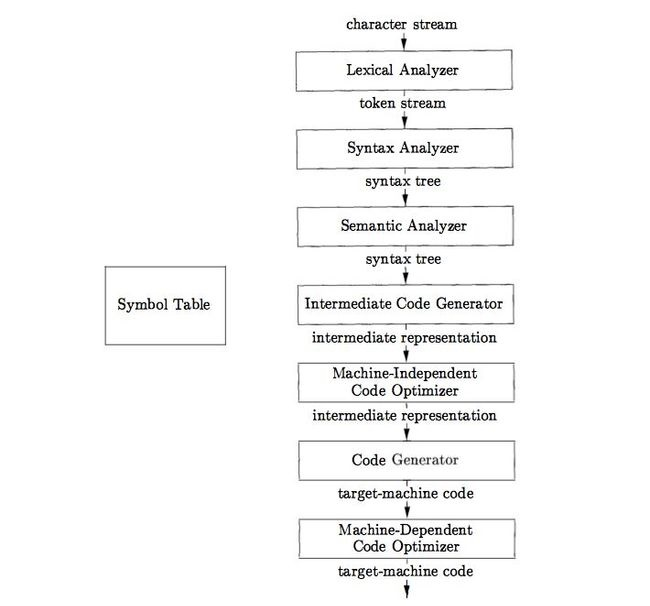
\includegraphics[width=1\textwidth]{Pictures/compiler_phases.jpg}
\end{center}
\caption{Glavne stopnje cevovoda prevajalnika~\cite{appel}}
\label{compilerPhases}
\end{figure}

Leksikalna analiza (angl. Lexical Analysis) je proces pretvarjanja niza znakov v niz žetonov. Žeton je niz znakov, ki mu je določen pomen. Program, ki izvaja lexikalno analizo se imenuje lekser (angl. Lexer). Lexer je običajno združen s parserjem, s katerim skupaj analizirata sintakso programskega jezika.


% FORMALNA GRAMATIKA ===================================================
\chapter{Gramatika} % (formal grammar)
\label{chOpis}
Programski jezik je opisan z kombinacijo semantike in gramatike. Semantika določa pomen vsakega konstrukta, ki je možen v programskem jeziku, gramatika pa določa strukturo konstrukta.\cite{Introduc96:online}
Gramatika - lahko tudi formalna gramatika - je predstavljena kot skupek produkcijskih pravil. Pravila opisujejo, na kakšen način lahko tvorimo nize, da ustrezajo veljavni sintaksi jezika. Gramatika sama po sebi ne opisuje pomena nizov, opisuje le njihovo obliko. S pomočjo gramatike lahko predstavimo določen program v obliki sintaksnega drevesa.

% TODO: Prosim da drugače napišeš tale stavek.
Gramatika je sestavljena iz niza simbolov. Vsak simbol je lahko končen ali nekončen. Končen pomeni, da je žeton abecede nizov programskega jezika. Lahko pa je nekončen kar pomeni, da se pojavi na levi strani določenega pravila. Noben žeton pa se ne more pojaviti na levi strani produkcijskega pravila.~\cite{Appel:2002}
\\

% BNF in EBNF razložena
\begin{itemize}
\item \textbf{Backus-Naur oblika (BNF)} % (Backus-naur Form) 
\\ 
Backus-Naur oblika ali tudi Backusova normalna oblika je notacijska tehnika za kontekstno neodvisne gramatike. Pogosto se uporablja za opisovanje sintakse jezika v računalništvu. Uporablja se pri: programskih jezikih, formatih dokumentov, naborih ukazov in komunikacijskih protokolih.~\cite{Backus:online}  

% TODO
% Primer preproste gramatike
% Question: Ali moram tudi tukaj citirati, da sem vzel iz vikipedije primer?
% Prosim, popravi tale primer. To je krneki. Tale primer gramatike sploh ni pravilen. to ni gramatika!
\begin{lstlisting}[caption={Primer preproste gramatike v BNF obliki},captionpos=b,label={lst:grammarBNFExample}, basicstyle=\small]
		<exp> ::= <exp> "+" <exp>
		<exp> ::= <exp> "*" <exp>
		<exp> ::= "(" <exp> ")"
		<exp> ::= "a"
		<exp> ::= "b"
		<exp> ::= "c"
\end{lstlisting}

\item \textbf{Razširjena Backus-Naur oblika (EBNF)} % (Extended Backus-naur Form)  
\\
Vsaka gramatika definirana v EBNF obliki je lahko predstavljena v BNF obliki, vendar so običajno gramatike nato daljše.~\cite{Extended22:online} 
Razširjena Backus-Naur oblika gramatike je družina metasintaksnih notacij, ki se uporabljajo za izražanje kontekstno neodvisne slovnice (gramatike). 

% TODO
% Primer preproste gramatike
% Question: Ali moram tudi tukaj citirati, da sem vzel iz vikipedije primer?
% Prosim, popravi tale primer. To je krneki. Tale primer gramatike sploh ni pravilen. to ni gramatika!
\begin{lstlisting}[caption={Primer preproste gramatike v EBNF obliki},captionpos=b,label={lst:grammarEBNFExample}, basicstyle=\small]
		Exp ::= Exp "+" Exp
			| Exp "*" Exp
			| "(" Exp ")"
			| "a"
			| "b"
			| "c"
\end{lstlisting}

\item \textbf{Povečana Backus-Naur oblika (ABNF)} % (Extended Backus-naur Form)  
% TODO: dodaj besedilo

\end{itemize}

% Obrazložitev primera gramatike
Izvorni kodi [\ref{lst:grammarBNFExample}] in [\ref{lst:grammarEBNFExample}] vsebujeta preprost primer gramatike artimetičnega izraza, ki je sestavljen iz operatorjev množenja in seštevanja, zapisanega v različnih oblikah gramatike.

% Primer zgornje gramatike v obliki sintaksnega drevesa
\begin{figure}[h!]
\centering
\begin{tikzpicture}[nodes={draw, circle}, 
level 1/.style={sibling distance=4cm},
level 2/.style={sibling distance=2cm},
level 3/.style={sibling distance=1cm}]
\node{+}
	child { node {expr} 
		child { node {a} }
	}
    child { node {expr} 
        child { node {(} }
        child { node {expr} 
        	child { node {b} }
        	child { node {*} }
        	child { node {c} }
        }
        child { node {)} }
    };
\end{tikzpicture}
\caption{Primer zgornje gramatike v obliki sintaksnega drevesa}
\label{grammarExampleSyntaxTree}
\end{figure}


\section{Kontekstno neodvisna gramatika} % (Context-Free Grammar)
Kontekstno neodvisna gramatika je določen tip formalne gramatike. Vsebuje produkcijska pravila, ki opisujejo vse možne nize za podan formalni jezik. Produkcijska pravila so preproste zamenjave. V CFG-ju je lahko vsako produkcijsko pravilo lahko le tipa:
% TODO: dodaj opis pri vsakem itemu
\begin{itemize}
\item Ena proti ena 
\item Ena proti mnogo
\item Ena proti nič
\end{itemize}

Jeziki, ki so generirani s pomočjo kontekstno neodvisne gramatike, se imenujejo kontekstno neodvisni jeziki (Context-Free Languages ali CFL). Različno zapisani CFG-ji lahko generirajo enak kontekstno neodvisni jezik. Zelo dober primer uporabe CFG-ja je pri XML (eXtensible Markup Language), ki uporablja definicijo tipa dokumenta (Document Type Definition ali DTD). V računalniški znanosti je popularen zapis CFG-ja kot BNF.

\section{Deterministična kontekstno neodvisna gramatika} % (Deterministic Context-Free Grammar)
Je podmnožica kontekstno neodvisne gramatike, ki generira deterministično neodvisen programski jezik (angl. \textit{Deterministic Context-Free Language ali DCFL}). DCFG-ji so vedno nedvoumni in so pomemben podrazred nedvoumnih CFG-jev. So tudi zelo praktični, saj so lahko parsani v linearnem času. Parser je lahko celo avtomatsko generiran iz gramatike z uporabo generatorja parserjev (Yacc, Antlr, Bison, JavaCC).

\section{Dvoumna gramatika} % (Ambigous Grammar)
Dvoumna gramatika je kontekstno neodvisna gramatika za katero lahko obstaja niz, ki ima več kot eno najbolj levo izpeljavo ali parsno drevo. Pri nedvoumni gramatiki, pa ima lahko vsak niz le unikatno najbolj levo izpeljavo ali parsno drevo. Mnogo programskih jezikov dovoli tako dvoumne kot nedvoumne gramatike vendar nekateri programski jeziki pa le nedvoumne. 
% TODO: dodaj, ker še nisi vse dopisal.

\section{Razčlenjevalno izrazna gramatika} % (Parsing Expression Grammar - PEG)
Je tip analitično formalne gramatike kar pomeni, da opisuje formalni jezik v odvisnosti od množice pravil za prepoznavanje nizov v jeziku. Razčlenjevalno izrazna gramatika (Parsing Expression Grammar ali PEG) je zelo povezana z družino odzgoraj-navzdol parsnih jezikov. Sintaktično PEG izgleda zelo podobno kot CFG vendar imajo DRUGAČNO interpretacijo. Izbirni operator izbere prvo ujemanje v PEG, medtem ko je izbira dvoumna pri CFG. Ta način je bližje temu, kako so prepoznani nizi v praksi s pomočjo rekurzivno spustnega parserja.
%TODO: Tole zgoraj ni dobro napisano!


% PARSER ===================================================
\chapter{Sintaksna analiza} % (Syntax Analyzer or Parser)
\label{chSyntaxAnalysis}
Parsanje oziroma sintaksna analiza je proces analiziranja niza simbolov (žetonov) ali ustrezajo pravilom formalne gramatike. Sintaksna analiza dobi iz leksikalne analize kot vhod niz simbolov iz katerih nato zgradi sintaksno drevo. 


\begin{figure}[h!]
\begin{center}
\makebox{\textless žeton, leksem, lokacija\textgreater}
\caption{Prikaz strukture posameznega simbola~\cite{pearson}}
\label{strukturaVhodnihPodatkov}
\end{center}
\end{figure}

Spodaj je prikazan primer [\ref{primerPreprostegaPrograma}] preprostega programa za pitagorov izrek in njegova drevesna struktura za sintaktično analizo [\ref{sintaksnoDrevo}].

\begin{figure}[h!]
\begin{center}
\[ c^2 = a^2 + b^2 \]
\caption{Primer programa za pitgorov izrek}
\label{primerPreprostegaPrograma}
\end{center}
\end{figure}


% TODO: Mogoče poskusi z gramatiko od Antlrja?
\begin{figure}[h!]
\begin{center}
\textless SPREMENLJIVKA, 'c', [1:1-1:1]\textgreater\\
\textless POTENCA, '\^{}', [1:2-1:2]\textgreater\\
\textless KONSTANTA, '2', [1:3-1:3]\textgreater\\
\textless ENAČAJ, '=', [1:4-1:4]\textgreater\\
\textless SPREMENLJIVKA, 'a', [1:5-1:5]\textgreater\\
\textless POTENCA, '\^{}', [1:6-1:6]\textgreater\\
\textless KONSTANTA, '2', [1:7-1:7]\textgreater\\
\textless PLUS, '+', [1:8-1:8]\textgreater\\
\textless SPREMENLJIVKA, 'b', [1:9-1:9]\textgreater\\
\textless POTENCA, '\^{}', [1:10-1:10]\textgreater\\
\textless KONSTANTA, '2', [1:11-1:11]\textgreater\\
\caption{Seznam simbolov za program [\ref{primerPreprostegaPrograma}]}
\label{seznamSimbolov}
\end{center}
\end{figure}

\begin{figure}[h!]
\begin{center}
\begin{forest}
  for tree={l+=0.1cm} % increase level distance
  [{=}
    [\^{}[c][2]]
    [+[\^{}[a][2]][\^{}[b][2]]]
  ] 
\end{forest}
\caption{Sintaksno drevo sestavljeno iz simbolov [\ref{seznamSimbolov}]}
\label{sintaksnoDrevo}
\end{center}
\end{figure}

% TODO: dodaj še opis Extended gramatike (Extended BNF)


% PARSERS ===================================================
\chapter{Vrste razčlenjevalnih metod}
\label{chParsingStrategies} % tale labela je zato, da lahko chapter referenciraš v kodi

Razčlenjevalniki tipa od zgoraj navzdol razpoznajo oziroma razčlenijo vhod iz oblike programskega jezika v notranjo predstavitev tako, da ujema prihajoče simbole v produkcijska pravila. Produkcijsko pravila so definirana z BNF. Spodaj so našteti in opisani različni parserji, ki delujejo po principu od zgoraj navzdol.



\begin{table}
\label{tbl:ParsersTopDown}
\centering
\begin{tabular}{l *{8}c}
\toprule
     & \rotbf{LL(*)} 
     & \rotbf{LL(1)} 
     & \rotbf{LL(k)} 
     & \rotbf{ALL(*)} 
     & \rotbf{Pred-LL(k)} 
     & \rotbf{\specialcell{Packart\\parser\\(PEG)}} 
     & \rotbf{\specialcell{Earley\\parser}} 
     & \rotbf{\specialcell{RDP-\\Handwritten}} \\
\midrule
%\specialcell{Assembly\\language} & 1 & 2 & 3 & 4 & 5 & 6 & 7 & 8 \\
\specialcell{Zbirni\\jezik} &  &  &  & Antlr4 & Antlr3 &  &  &  \\
\specialcell{Action\\script} &  &  &  & Antlr4 &  &  &  &  \\
Ada &  & Coco/R &  & Antlr4 &  &  &  &  \\
Basic &  &  &  & Antlr4 &  &  &  &  \\
C &  & Coco/R &  & Antlr4 & Antlr3 &  &  & \specialcell{GCC4\\CLang\\APG} \\

\bottomrule
\end{tabular}

\caption{Tabela odzgoraj-navzdol razčlenjevalnih metod v povezavi z programskimi jeziki in razčlenjevalniki}
\end{table}



% PARSERS ===================================================
\chapter{Razčlenjevalniki} % (Compiler or Parser)
\label{chParsers}
random text

\section{GCC}
random text

\section{CLion}
random text

\section{Roslyn}
random text

\section{Esprima}
random text

\section{Nashorn}
random text

\section{Chrome V8}
random text

\section{SpiderMonkey}
random text

\section{Rhino}
random text


% PARSER GENERATOR ===================================================
\chapter{Generatorji razčlenjevalnikov} % (Compiler Compiler or Parser Generator)
\label{chParserGenerators}
random text

\section{Antlr}
random text

\subsection{Programski jeziki}
random text

\subsection{Gramatika}
random text

\subsection{ALL(*)}
random text

\subsection{Pred-LL(k)}
ranodm text


\section{Yacc}
random text

\begin{itemize}  
\item Lex
% TODO: write text
\item Flex
% TODO: write text
\end{itemize}

\section{GNU Bison}
random text

\section{JavaCC}
random text



% CONCLUSION =====================================================
\chapter{Sklepne ugotovitve}  % Tukaj pač poveš do kakšnega zaključka si prišel, kateri so najbolj uporabni parserji in zakaj.
\label{chConclusion}
random text



\newpage %dodaj po potrebi, da bo številka strani za Literaturo v Kazalu pravilna!
\ \\
\clearpage
\addcontentsline{toc}{chapter}{Literatura}
\bibliographystyle{plain}
\bibliography{literatura}


\end{document}

